\documentclass[a4paper,11pt]{article}

\usepackage[utf8]{inputenc}

\usepackage{pgfplots}

\usepackage{minted}

\begin{document}

\title{
    \textbf{A heap or priority queue}
}
\author{Mahdi Nazari}
\date{October 2022}

\maketitle
\section*{Priority queue as a linked list}
In a priority queue each element will be ordered regard to its priority which can be define in different ways. In this assignment will priority be defined as the value of element such that the element with a smaller value has higher priority and should be placed in the front of the queue. The simplest way to implement a priority queue is as a linked list. The elements with smaller values are placed earlier in the queue and closer to the head of linked list. The fundamentals operations in priority queue are adding an element in the queue and removing an element with highest priority. Implementation of add- and remove methods in this priority queue can be done in two ways. First implementation can be to add an element in the queue in a constant time e.g. adding elements at the end of the queue and removing the element with highest priority, first by identifying it in the queue and then removing it which would require a execution time of O(n) type. Second implementation can be to add an element in the queue in order such that the element with higher priority should be placed closer to the front of the queue which requires that each element in the queue after adding should be moved to its right place which can be done in an execution time of O(n) type and removing the element with highest priority can be done in a constant time since we know that the queue is ordered and the element with highest priority would be the element in the head of the linked list.\newline
These two different implementations give us possibility to choose if we want add an element in the priority queue in constant time and we are not using the remove method that much then the first implementation can be suitable. But if we do not care about the time to add an element in the priority queue and we just want get the element with the highest priority in constant time then the second implementation is useful. These two implementations will be benchmarked in the last section.     



\section*{Heap as a linked structure}
Priority queue can be also implemented as a heap. Heap can be seen as a binary tree but there is a difference. In a heap the elements are ordered in the tree such that the elements with higher priority are closer to the root and the root has the highest priority. The root in a heap has two branches which are two heaps in their own. Highest priority in this assignment means that an element with the smallest value but it could be the largest value as well. Again two essential operations in a heap are add and remove operations. We want have a balanced heap therefore we need to keep track of where we should add an element in the heap. We construct the heap such that each node has a variable "size" that keeps track of how many elements there are in the heap with this node as the root. To add an element in the heap we need to fulfil two requirements, one the element should be placed in the right place such that the heap keeps its order and the element should be placed in that branch which has lower number of nodes. To remove an element from the heap is simple since the highest priority is always the root of the heap but we need then to rearrange the elements to have the next smallest value as the root of the heap.\newline
To compare a priority queue as a linked list to a priority queue as a heap we know that heap is constructed as a binary tree and this means adding an element to the heap can be performed in a time of O(log n) type. Removing element from the heap is divided in two parts first removing the root which is constant and rearrangement of the heap which in worst case can be performed in a time of O(log n) type. In other words heap implementation of priority queue has add and remove methods which both can be performed in a time of O(log n) type, but linked list implementation of priority queue had either add method with a constant time complexity and remove method with a linear time complexity or add method with a linear time complexity and remove with a constant time complexity.\newline
Another method was implemented in the heap which is called "push". This method performs such that it takes the root which has the highest priority and increment it by a value which means that the root changes its priority and should be replaced in the heap in a way to keep the heap ordered. Push operation is efficient in a situation we want do some operations on the highest priority in the heap and return the result back to the heap which in worst case can be done in a time of O(log n) instead of first removing the root which can be done in a time of O(log n) type and then adding the result back to the heap by a time of O(log n) type. We will take some statistics about the push operation and will prove if the time complexity of the push operation is always O(log n) type or less than that. We construct the push method such that it has a variable "depth" which will return the lowest level that the push method has reached. \newline
We know that the (log n) is the height of the heap and an operation has a time complexity of O(log n) if it reaches the lowest level in the heap. We assume that in the most cases push operation has a time complexity less than O(log n). We know that add operation reaches always the bottom level in the heap. We reconstruct the add operation such that it returns a value which shows the depth or the lowest level of the heap that the add operation had to reach to add an element. Push and add methods are benchmarked and the result will be rapported in the last section.          

\section*{Heap as an array}
There is another implementation of the heap which is based on an array, the elements with higher priority is closer to the start of the array which means the element with the highest priority is at index 0 in the array. We need again add and remove methods to perform these operations. This time heap is constructed by an array and a pointer "index" which keeps track of the last element in the heap. To add an element we set the element at the end of the array and to keep the heap ordered we compare this new added element with its parent and if its value is less than its parents it has to swap with its parent. This procedure is called "bubble" and goes on until it reaches a situation where this new added element is in the right place in the heap. We know that if an element is placed at index n in the array then its parent is at index (n-1/2). The add method is as follows:

\begin{verbatim}
 public void add(int item){
       array[index++]=item;
       bubbla(array); 
       }
  public void bubbla(int[]array){
       int child = index - 1;
       int parent = (child-1)/2;
       while(array[child] < array[parent] && parent > -1){
        int temp = array[child];
        array[child] = array[parent];
        array[parent] = temp;
        child = parent;
        parent = (child-1)/2;}
    }
\end{verbatim}  

To remove an element in the heap we know that the element at index 0 should be returned. Last element in the array should be copied to the index 0 and decrement the pointer index by one. Then the last element that now is replaced at index 0 should move to its right place to keep the heap ordered. To do this a procedure which will be called "sink" will start and the element at index 0 will be compared with its children and if it has a value larger than its children it has to swap with the child with the smallest value. Sink procedure continues until the element at index 0 is in the right place in the heap. We know that if an element is at index n in the array its children are at index 2n+1 and 2n+2.

\section*{Benchmark}
In this part, the results from benchmarking of different implementations will be presented.  

\subsection*{Priority queue as a linked list}
A benchmark was set to compare the execution time of (Implementation1) priority queue as a linked list with an add operation of O(1) type and remove operation of O(n) type in comparison to (Implementation2) a priority queue as a linked list with an add operation of O(n) type and remove operation of O(1) type. The benchmark was set so that the same randomly chosen sequence of elements was added and removed by Impl.1 and Impl. 2 and the execution time was calculated. To get a clear picture the size of sequence was increased a few times and the result is as in the table below.

 \begin{table}[h]
\begin{center}
\begin{tabular}{l|S|l}
\textbf{Number } & \textbf{Impl. 1}  & \textbf{Impl. 2} \\
\hline
  100      &  12 us &6 us\\
  200      &  47 us & 22 us\\
  300      &  101 us& 49 us\\
  400      &  179 us & 90 us\\
  500      &  281 us & 141 us\\
  600      &  401 us & 204 us\\
\end{tabular}
\caption{The execution time to add and remove different numbers of elements by Impl.1 and Impl. 2.}\newline
\label{tab:table1}
\end{center}
\end{table}\newline     
Comments: From the result can we conclude that the Impl.2 which has an add operation of O(n) type and a remove operation of O(1) type is totally more efficient regard to the execution time than the Impl.1.
 
\subsection*{Add and push methods in a heap as a linked structure}
In this part we will benchmark add and push method in a heap as a linked structure. A benchmark was set so that 64 randomly chosen elements(from 0 to 100) was added to the heap and then a randomly chosen sequence(from 10.....20) was added to the heap and pushed the root by. The add and push methods returns a value that shows the depth of the heap that they had reached. To show a clear picture of differences of these two methods the average of depth value was calculated for each sequence of elements that has been added and pushed. Result is as the table below.
  \begin{table}[h]
\begin{center}
\begin{tabular}{l|S|l}
\textbf{Number } & \textbf{Push}  & \textbf{Add} \\
\hline
  100      &  4 & 6 \\
  1000      &  4& 8\\
  10000      &  4 & 11 \\
  100000      &  4  & 14 \\
  1000000      &  4 & 17 \\
\end{tabular}
\caption{The average depth of the heap that push and add operation had to go down to}\newline
\label{tab:table1}
\end{center}
\end{table}\newline  
Comments: The result shows that push operation in average has to go down to level fourth for pushing(incrementing) the root by 100 elements from 10 to 20 and this average depth seems to be the same even if we push the root by 1000000 elements from 10 to 20. This means that the time complexity of the push operation in average is even less than the O(log n). Because the (log n) is the height of the heap and push operation seems to do not go to the bottom of the heap in most cases. In add operation the method has to go down to the bottom to add a new element and therefore the time complexity of add operation is O(log n) type.        

\subsection*{Heap as a linked structure VS heap as an array}
A benchmark was set so that a number of randomly chosen elements was added and removed by a heap as a linked structures and by a heap as an array. The execution time was calculated for adding and removing of each sequence. The graph below shows the result from benchmarking. 
\begin{center}
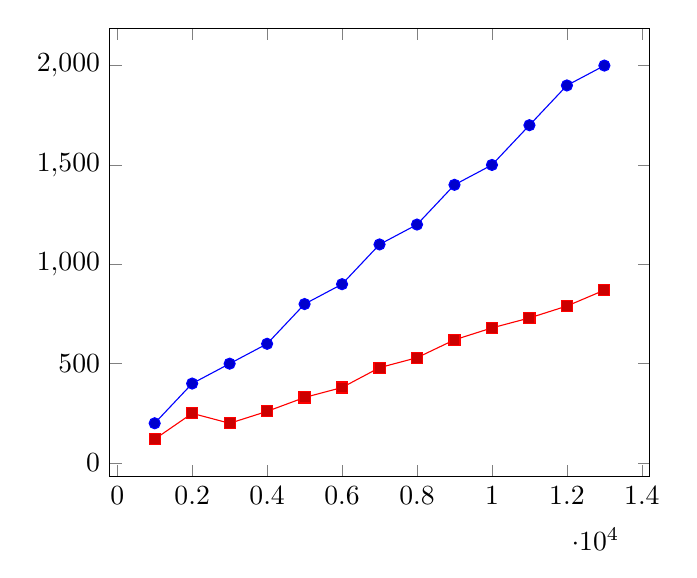
\begin{tikzpicture}
   \begin{axis}
    \addplot coordinates {
    (1000 ,200)
      ( 2000 ,400 )
      (3000,500)
      ( 4000, 600)
      ( 5000, 800)
       (6000, 900)
        (7000, 1100)
       ( 8000, 1200)
       (9000, 1400)
       (10000,1500)
        (11000,1700)
 	(12000,1900)
 	(13000,2000)         
    };
     \addplot coordinates {
      ( 1000 ,120 )
      ( 2000 , 250)
      (3000, 200)
      ( 4000, 260)
      ( 5000, 330)
       (6000, 380)
        (7000, 480)
       ( 8000, 530)
       (9000, 620)
       (10000, 680)
        (11000,730)
 	(12000,790)
 	(13000,870)
           };
      \end{axis}\newline
\end{tikzpicture}\newline
\caption{Graph 1: The result from benchmarking heap as a linked structure(blue graph) and heap as an array(red graph), x-axis is size of data sets, y-axis is execution time in us. }
\end{center}\newline
Comments: adding and removing elements in both implementations of heap are an O(log n) type, so adding and removing totally has a time complexity of 2*O(log n) which can be still simplified to O(log n).  The graph of the heap as an array(red graph) shows this clear. But the graph of heap as a linked structure(blue graph) is closer to be an O(n) type. This can be because of the benchmark maybe was not performed perfectly and there are some other factors that impacts the execution time that has not been discovered. The obvious result is that the array implementation of the heap is more efficient than the linked structures implementation.  



\end{document}
